% !TEX TS-program = pdflatex
% !TEX encoding = UTF-8 Unicode

% This is a simple template for a LaTeX document using the "article" class.
% See "book", "report", "letter" for other types of document.

\documentclass[11pt]{article} % use larger type; default would be 10pt

\usepackage[utf8x]{inputenc}
\usepackage[T1]{fontenc}
\usepackage[polish]{babel}
\usepackage{hyperref}
\usepackage{graphicx} 


%%% Examples of Article customizations
% These packages are optional, depending whether you want the features they provide.
% See the LaTeX Companion or other references for full information.

%%% PAGE DIMENSIONS
\usepackage{geometry} % to change the page dimensions
\geometry{a4paper} % or letterpaper (US) or a5paper or....
% \geometry{margin=2in} % for example, change the margins to 2 inches all round
% \geometry{landscape} % set up the page for landscape
%   read geometry.pdf for detailed page layout information

\usepackage{graphicx} % support the \includegraphics command and options

% \usepackage[parfill]{parskip} % Activate to begin paragraphs with an empty line rather than an indent

%%% PACKAGES
\usepackage{booktabs} % for much better looking tables
\usepackage{array} % for better arrays (eg matrices) in maths
\usepackage{paralist} % very flexible & customisable lists (eg. enumerate/itemize, etc.)
\usepackage{verbatim} % adds environment for commenting out blocks of text & for better verbatim
\usepackage{subfig} % make it possible to include more than one captioned figure/table in a single float
% These packages are all incorporated in the memoir class to one degree or another...

%%% HEADERS & FOOTERS
\usepackage{fancyhdr} % This should be set AFTER setting up the page geometry
\pagestyle{fancy} % options: empty , plain , fancy
\renewcommand{\headrulewidth}{0pt} % customise the layout...
\lhead{}\chead{}\rhead{}
\lfoot{}\cfoot{\thepage}\rfoot{}

%%% SECTION TITLE APPEARANCE
\usepackage{sectsty}
\allsectionsfont{\sffamily\mdseries\upshape} % (See the fntguide.pdf for font help)
% (This matches ConTeXt defaults)

%%% ToC (table of contents) APPEARANCE
\usepackage[nottoc,notlof,notlot]{tocbibind} % Put the bibliography in the ToC
\usepackage[titles,subfigure]{tocloft} % Alter the style of the Table of Contents
\renewcommand{\cftsecfont}{\rmfamily\mdseries\upshape}
\renewcommand{\cftsecpagefont}{\rmfamily\mdseries\upshape} % No bold!

%%% END Article customizations

%%% The "real" document content comes below...

\title{MNUM Projekt, zadanie 1.19}
\author{Monika Pawluczuk, nr indeksu 246428}
%\date{} % Activate to display a given date or no date (if empty),
         % otherwise the current date is printed 

\begin{document}
\maketitle

\section{Zadanie 1}

\subsection{Treść polecenia}

Proszę napisać program wyznaczający dokładność maszynową komputera i wyznaczyć ją na swoim komputerze.

\subsection{Zastosowane algorytmy}

Dokładność maszynowa to maksymalny błąd względny reprezentacji zmiennoprzecinkowej równy 2 do -t, gdzie t to liczba bitów mantysy - a więc zależny wyłącznie jej liczby. Zgodnie z przyjętą konwencją, będę go oznaczać jako eps.
Równoważną definicją jest również najmniejsza dodatnia liczba maszynowa g taka, że zachodzi relacja 
\begin{equation}
fl(1 + g) > 1, tzn. eps = min \{  g \in M : fl(1 + g) > 1, g > 0\}
\end{equation}
Zgodnie z drugą definicją, przyjmę początkowy eps jako 1. Będę zmniejszać eps o połowę w każdej iteracji, dopóki eps + 1 > 1 (czyli eps > 0). Wyjście z pętli będzie oznaczało, że znaleźliśmy najmniejszy możliwy błąd.

\subsection{Implementacja użytych algorytmów}

\begin{verbatim}
function [ t, eps ] = machinePrecision()
%MACHINEPRECISION Return computer's machine precision
%   Return the least numeric value that is threated by the computer as
%   value above 0.
    eps = 1.0;
    t = 0;
    while (1.0 + eps/2.0 > 1.0)
        eps = eps/2.0;
        t = t + 1;
    end
    [t, eps];
end

\end{verbatim}

\subsection{Otrzymane wyniki oraz komentarz}

\begin{verbatim}
>> [t, eps] = machinePrecision()
t =
    52
eps =
   2.2204e-16
>> eps + 1.0 > 1.0
ans =
     1
\end{verbatim}
A więc liczba bitów mantysy to 52, natomiast dokładnośc maszynowa wynosi 2.2204e-16. Jest to wynik zgodny ze standardem IEEE 754 dla liczb zmiennoprzecinkowych podwójnej precyzji.

\section{Zadanie 2}

\subsection{Treść polecenia}

Proszę napisać program rozwiązując układ n równań liniowych Ax=b wykorzystując podaną metodę. Proszę zastosować program do rozwiązania podanych niżej układów równań dla rosnącej liczby równań n = 10, 20, 40, 80, 160, …. Liczbę tych równań proszę zwiększać do momentu, gdy czas potrzebny na rozwiązanie układu staje się zbyt duży/metoda zawodzi.
Metoda: Eliminacja Gaussa z częściowym wyborem elementu podstawowego, 3 zestawy danych.
Dla każdego rozwiązania proszę obliczyć błąd rozwiązania (liczony jako norma residuum) i dla każdego układu równań proszę wykonać rysunek zależności tego błędu od liczby równań n.

\subsection{Zastosowane algorytmy}
Dla przypomnienia, podstawowy algorytm eliminacji Gaussa dzieli się na dwa etapy:

1. Eliminacja zmiennych - w wyniku przekształceń macierzy A i wektora b otrzymamy równoważny układ równań z macierzą trójkątną górną.

2. Postępowanie odwrotne (ang. back-substitution) - stosujemy algorytm rozwiązania układu z macierzą trójkątną.

Metoda eliminacji Gaussa z częściowym wyborem elementu podstawowego
1. Korzystając z metody podstawowej, również dzielimy działanie na k kroków, w każdym działając na kolumnie (k). Modyfikacja polega na tym, że wybieramy taki element 
\begin{equation}
a_{jk}^{(k)} (k <= j <=n),
\end{equation} 
dla którego moduł jest największy. Oznaczmy go jako i.

Następnie zamieniamy i-ty wiersz z k-tym i stosujemy dalej standardowy algorytm.
Takie zachowanie pozwala na uniknięcie sytuacji blokującej, kiedy 
\begin{equation}
a_{kk}^{(k)} = 0 
\end{equation}
Stosowanie modyfikacji odrzuca taką możliwość, ponieważ z definicji zakładamy, że macierz A jest nieosobliwa.

\subsection{Implementacja użytych algorytmów}

\subsubsection{Generowanie macierzy A i b dla każdego zestawu danych}

\begin{verbatim}

function [ A , B ] = generateMatrix( option, equations )
%GENERATEMATRIX Generowanie macierzy z danymi
%   option - który zestaw danych generujemy (1,2 lub 3)
%   equations - liczba rownan

% empty A array with dimensions [equations x equations]
A = zeros(equations);
% empty B array with dimensions [equations x 1]
B = zeros(equations,1);

if (option == 1)
    for i = 1:equations
        % replace B[i,1] with appropriate values
        B(i,1) = 1.5 + 0.2*i;
        % replace A[i,j] with appropriate values
        for j = 1:equations
            if ( i == j ) 
                A(i,j) = 5;
            elseif ( i == j - 1 || i == j + 1 ) 
                    A(i,j) = 2;
            else A(i,j) = 0;
            end
        end
    end
end

if (option == 2)
    for i = 1:equations
        % replace B[i,1] with appropriate values
        B(i,1) = 1.0 + 0.2*i;
        % replace A[i,j] with appropriate values
        for j = 1:equations
            if ( i == j )  
                A(i,j) = 0.125;
            else
                A(i,j) = 3*(i - j) + 2;
            end
        end
    end
end

if (option == 3)
    for i = 1:equations
        % replace B[i,1] with appropriate values
        if (mod(i, 2) == 0)
            B(i,1) = 5 / (4 * i);
        else
            B(i,1) = 0;
        end
        % replace A[i,j] with appropriate values
        for j = 1:equations
            A(i,j) = 3 / (5 * (i + j + 1));
        end
    end
end
    
end

\end{verbatim}

\subsubsection{Generowanie układów równań do rozwiązania i rysowanie wykresów}

\begin{verbatim}
function [ ] = solveGauss( )
%SOLVEGAUSS Wygeneruj uklady rownan
%   Rozwiaz rownania przy pomocy eliminacji Gaussa z czesciowym wyborem
%   elementu podstawowego dla roznej liczby rownan.
%   Dla kazdego zestawu danych generuje wykres zaleznosci bledu
%   od liczby rownan.

% zestaw danych od 1 do 3
for i = 1 : 3
    iterations = 6;
    results = zeros(iterations, 1);
    iterationsTable = zeros(iterations, 1);
    for n = 1 : iterations
        equations_number = 2^n * 10;
        [ A, b ] = generateMatrix(i, equations_number);
        r = gaussElimination(A, b);
        results(n) = r;
        iterationsTable(n) = equations_number;
    end
    [iterationsTable results]
    titleString = sprintf('Zestaw danych: %d', i);
    figure()
    plot(iterationsTable, results)
    title(titleString)
    xlabel('Ilosc iteracji')
    ylabel('Norma residuum')
end

end

\end{verbatim}

\subsubsection{Metoda eliminacji Gaussa z częściowym wyborem elementu podstawowego}

\begin{verbatim}
function [ r ] = gaussElimination( A, b)
%GAUSSELIMINATION Eliminacja Gaussa
%   Metoda z czesciowym wyborem elementu glownego

% Dane testowe z ksiazki
%A = [3 1 6;2 1 3;1 1 1];
%b = [2;7;4];

n = size(A, 1);

M = [A b];
X = zeros(n, 1);

% dokonujemy n - 1 krokow (przeksztalcen),
% jednoczesnie kolumna na ktorej operujemy
for k = 1 : n - 1
    main_element = 0;
    ik = M(k,k);
    
    % wybieramy element glowny
    for j = k + 1 : n
        if (abs(M(j,k)) > main_element)
            main_element = abs(M(j,k));
            ik = j;
        end
        
        % wybralismy element maksymalny w kolumnie k 
        % i zapisalismy w jakim byl rzedzie w ik
        % teraz zamieniamy rzad k z ik
        if (ik ~= k)
            temp = M(k,:);
            M(k,:) = M(ik,:);
            M(ik,:) = temp;
        end
    end
    
    % zakladamy ze M(ik,k) != 0, bo A jest nieosobliwa
    % jesli jest, to wkradl sie blad
    if (M(ik, k) == 0)
        disp('Macierz A osobliwa - nie mozna rozwiazac. Blad programu.');
        break
    end
    
    column_factor = M(k, k);
    % wyliczamy wspolczynniki do przeksztalcenia wierszy
    for r = k + 1 : n
        l_rk = M(r, k) / column_factor;
        % przemnazamy wiersze po kolei w_i = w_i - l_i:i-1*w_i-1
        for i = k : n + 1
            M(r,i) = M(r, i) - l_rk*M(k, i);
        end
        % nasza macierz wynikowa M to polaczenie macierzy L i U
        % podstawiamy elementry macierzy L w miejsce wyzerowanych
        % elementow z A aby zaoszczedzic pamiec
        M(r,k) = l_rk;
    end
end

% "odzyskujemy" wektor b
b = M(:, n + 1);

% nasza macierz M dzielimy na macierze L i U
% macierz L - diagnostycznie
L = eye(n);
U = zeros(n);
% iteracja po kolumnach
for i = 1 : n
    % iteracja po wierszach
    for k = 1 : n
        if (k >= i + 1) 
            L(k, i) = M(k, i);
        else
            U(k, i) = M(k, i);
        end 
    end
end

% rozwiazanie ukladu
% metoda back-substitution 
% czyli idziemy od ostatniego wiersza, gdzie mamy od razu rozwiazanie xn
% pierwsze dwa elementy wyliczamy "recznie"
X(n) = b(n) / U(n, n);
X(n - 1) = (b(n - 1) - U(n - 1, n) * X(n)) / U(n - 1, n - 1);

% pozostale elementy
for k = 2 : n - 1
    % wlasciwe k 
    k1 = n - k;
    suma = 0;
    for j = k1 + 1 : n
        suma = suma + U(k1, j)*X(j);
    end
    X(k1) = (b(k1) - suma) / U(k1, k1);
end

% obliczenie bledu rozwiazania
% jako normy residuum
% liczymy residuum
r = b - U * X;
% norma druga residuum
r = r.^2;
r = sqrt(sum(r));

end
\end{verbatim}

\subsection{Otrzymane wyniki oraz komentarz}
\subsubsection{Tabele zależności normy residuum od liczby równań}
Zestaw danych nr 1

\begin{table}[h]
\begin{tabular}{|l|l|lll}
\cline{1-2}
Liczba iteracji & Norma residuum &  &  &  \\ \cline{1-2}
20             & 1.0878e-15            &  &  &  \\ \cline{1-2}
40             & 1.4043e-15            &  &  &  \\ \cline{1-2}
80            & 3.4111e-15                &  &  &  \\ \cline{1-2}
160            &  5.8072e-15              &  &  &  \\ \cline{1-2}
320            & 1.9352e-14               &  &  &  \\ \cline{1-2}
640            &  5.8342e-14              &  &  &  \\ \cline{1-2}
\end{tabular}
\end{table}

Zestaw danych nr 2

\begin{table}[h]
\begin{tabular}{|l|l|lll}
\cline{1-2}
Liczba iteracji & Norma residuum &  &  &  \\ \cline{1-2}
20             & 9.2264e-16           &  &  &  \\ \cline{1-2}
40             &  2.0150e-15            &  &  &  \\ \cline{1-2}
80            & 1.8007e-15                &  &  &  \\ \cline{1-2}
160            &  1.2627e-15              &  &  &  \\ \cline{1-2}
320            & 1.4925e-14               &  &  &  \\ \cline{1-2}
640            &  2.9782e-14              &  &  &  \\ \cline{1-2}
\end{tabular}
\end{table}

Zestaw danych nr 3

\begin{table}[h]
\begin{tabular}{|l|l|lll}
\cline{1-2}
Liczba iteracji & Norma residuum &  &  &  \\ \cline{1-2}
20             & 0.0425            &  &  &  \\ \cline{1-2}
40             & 0.1219            &  &  &  \\ \cline{1-2}
80            &  0.0794                &  &  &  \\ \cline{1-2}
160            &  0.8722              &  &  &  \\ \cline{1-2}
320            &  0.0454               &  &  &  \\ \cline{1-2}
640            &  0.4940              &  &  &  \\ \cline{1-2}
\end{tabular}
\end{table}

\subsubsection{Wykresy zależności normy residuum od liczby równań}
(Strony 9,10,11)
\begin{figure}
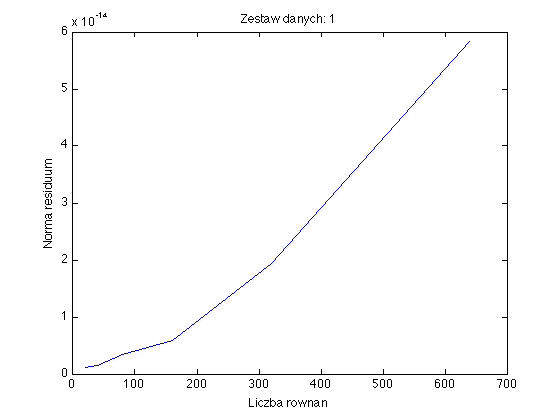
\includegraphics{zestaw1}
\end{figure}
\begin{figure}
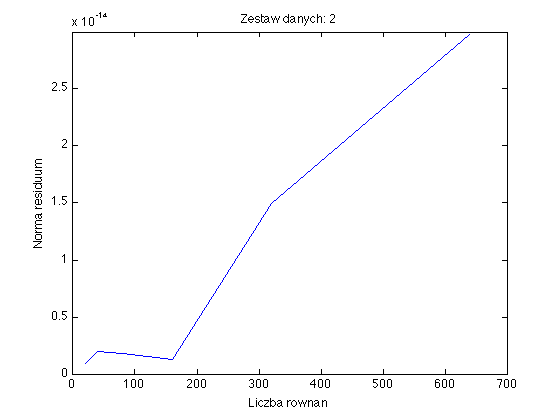
\includegraphics{zestaw2}
\end{figure}
\begin{figure}
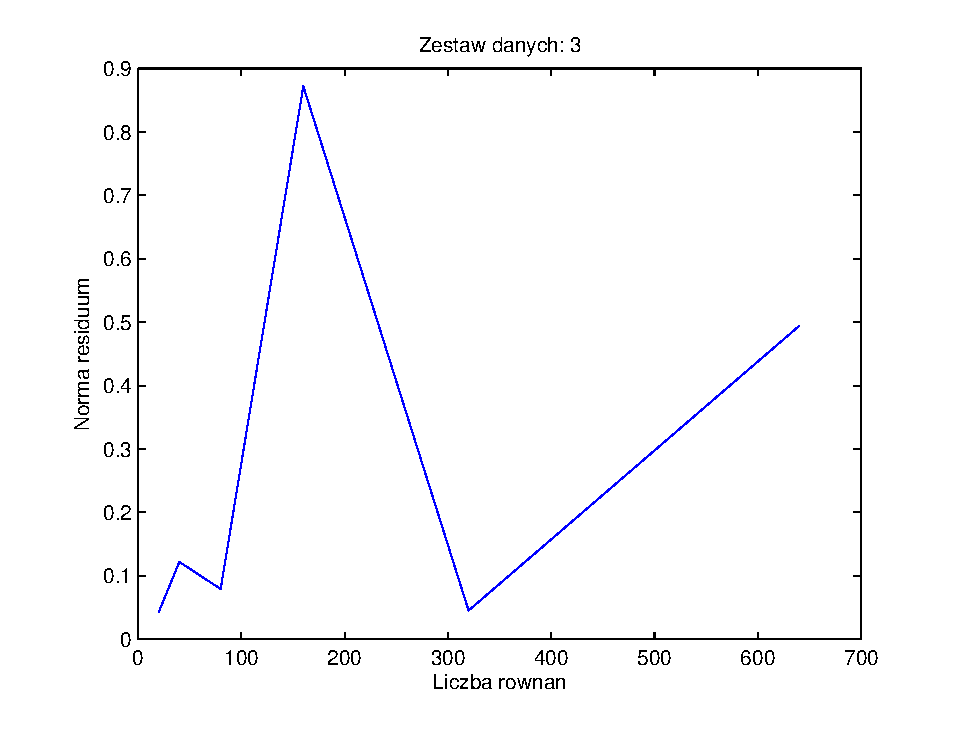
\includegraphics{zestaw3}
\end{figure}

\subsubsection{Wnioski}

Widać, że norma residuum dla ostatniego zestawu danych jest większa o kilkanaście rzędów w porównaniu do zestawu danych 1 i 2.

Widać, że dla zestawu danych 1 i 2 błąd nie ma granicy i rośnie wraz z ilością równań.
Wyraźne wahania poziomu residuum w zależności od liczby iteracji widać w zestawie trzecim, gdzie generowane były macierze bez zerowych elementów.

\section{Zadanie 3}

\subsection{Treść polecenia}

Proszę napisać program rozwiązujący układ n równań liniowych Ax=b wykorzystując metodę Jacobiego i użyć go do rozwiązania poniższego układu równań liniowych.

Proszę sprawdzić dokładność rozwiązania oraz spróbować zastosować zaprogramowaną metodę do rozwiązania układów równań z zadania 2.

\subsection{Zastosowane algorytmy}

Metoda Jacobiego jest metodą iteracyjną rozwiązywania układów równań liniowych. Polega na tym, że dokomponujemy macierz A na sumę trzech macierzy: L, D i U.
L jest macierzą poddiagnoalną, D - diagonalną, U - naddiagonalną.

Podstawiając owe macierze i przekształcając równanie, nasz układ równań można zapisać:
\begin{equation}
Dx = -(L + U)x +b
\end{equation}

Zakładamy, że macierz D jest nieosobliwa. Daje nam to możliwość zastosowania metody iteracyjnej:
\begin{equation}
x^{(i+1)} = -D^{-1}(L+U)x^{(i)} + D^{-1}b, i = 0,1,2,...
\end{equation}
co jest równoważne z:
\begin{equation}
x_{j}^{(i +1)} = - 1/d_{jj} * \sum_{k=1}^{n} (l_{jk} + u_{jk})x_{k}^{(i)} = b_{j}, j = 1,2,..,n
\end{equation}

Jakość metody zależy przede wszystkim od liczby iteracji, a więc warunkiem stopu jest wynik subiektywny, który nas zadowala.

\subsection{Implementacja użytych algorytmów}

\subsubsection{Generowanie macierzy i jej rozwiązywanie}

\begin{verbatim}

function [] = solveJacob( )
% solveJacob Generuje macierze i przekazuje do rozwiazania
% aby je rozwiazan metoda Jacobiego

N = 1000;

for i = 1 : 3
    for k = 3 : 10
        [A, b] = generateMatrix(i, k);
        Jacob(A, b, N);
    end
end

end

\end{verbatim}

\subsubsection{Implementacja metody Jacobiego}

\begin{verbatim}

function [] = Jacob( A, b, iterations )
%Jacob Rozwiazywanie ukladu rownan
%   metoda iteracyjna Jacobiego
% iterations - maksymalna liczba iteracji

% rzad macierzy A
n = size(A,1);

% rozbicie macierzy A = L + D + U:
% macierz naddiagonalna
U = triu(-A,1);
% macierz diagonalna
D = diag(diag(A));
% macierz poddiagonalna
L = tril(-A, -1);

Tj = inv(D)*(L+U);
cj = inv(D)*b;

% tolerancja - z gory ustalona
esp = 1e-10;
% zmienna do iteracji
k = 1;
% szukany wektor - zaczynamy od samych zer
x = zeros(n,1);


%warunek dostateczny zbieznosci metody jacobiego:
for i = 1 : n
   %dominacja wierszowa
   disp(i);
   dominacjaWierszowa = 1;
   for i = 1 : n 
    if ( abs(A(k,k)) < A(i, k) )
        dominacjaWierszowa = 0;
    end
   end
   if (dominacjaWierszowa == 1)
       disp('Warunek dominacji wierszowej spelniony')
   else
       disp('Warunek dominacji wierszowej nie jest spelniony')
   end
   
   %dominacja kolumnowa
   dominacjaKolumnowa = 1;
   for i = 1 : n 
    if ( abs(A(k,k)) < A(k, i) )
        dominacjaKolumnowa = 0;
    end
   end
   if (dominacjaKolumnowa == 1)
       disp('Warunek dominacji kolumnowej spelniony')
   else
       disp('Warunek dominacji kolumnowej nie jest spelniony')
   end
end
   
while k <= iterations
   x(:,k + 1) = Tj * x(:, k) + cj;
   
   if norm(x(:,k + 1) - x(:, k)) < esp
      disp('Osiagnieto zadany warunek stopu: ||x^(k+1) - x^(k)|| < esp dla wartosci:')
      disp('Liczba iteracji:');
      disp(k); 
      disp('x = ');
      disp(x(:,k + 1));
      break
   end
   k = k+1;
end

if ( norm(x(:,k + 1)- x(:, k)) > esp || k > iterations )
   disp('Nie udalo sie osiagnac warunku stop. Log:')
   disp('Esp:')
   disp(esp);
   disp('x = ');
   disp(x');
end

\end{verbatim}

\subsection{Otrzymane wyniki oraz komentarz}
\subsubsection{Wyniki dla danego układu równań}
\begin{verbatim}
>> A = [25 2 -18 1; 1 17 5 -8; -2 8 -21 5; 1 2 -1 13]

A =

    25     2   -18     1
     1    17     5    -8
    -2     8   -21     5
     1     2    -1    13

>> b = [5 46 184 2]'

b =

     5
    46
   184
     2
 
>> Jacob(A,b, 1000)
     1

Warunek dominacji wierszowej spelniony
Warunek dominacji kolumnowej spelniony
     2

Warunek dominacji wierszowej spelniony
Warunek dominacji kolumnowej spelniony
     3

Warunek dominacji wierszowej spelniony
Warunek dominacji kolumnowej spelniony
     4

Warunek dominacji wierszowej spelniony
Warunek dominacji kolumnowej spelniony
Osiagnieto zadany warunek stopu: ||x^(k+1) - x^(k)|| < esp dla wartosci:
Liczba iteracji:
    28

x = 
   -4.9584
    4.6385
   -6.6876
   -0.6928

\end{verbatim}

\subsection{Wyniki dla układów równań z zadania 2}
Udało się otrzymać wyniki dla każdego rodzaju danych dla macierzy o niewielkich rozmiarach.

Zestaw danych nr 1 ma najwieksze wartości na diagonali, a więc warunki dostateczne zbieżności zawsze są spełnione (zarówno dominacja wierszowa jak i kolumnowa).

W zestawie danych nr 3 dominacja wierszowa i kolumnowa nie zawsze była spełniona, i części układów nie udało się rozwiązać.

Liczba iteracji wahała się w granicach do ok. 100 dla tolerancji ustalonej na 1e-10.
Metoda ta działa zdecydowanie szybciej w porównaniu do metody z zadania drugiego, natomiast jest też mniej dokładna. Plusem tej metody jest możliwość ustalenia liczby iteracji, jednak wymaga ona ustalenia własnego warunku stopu (tolerancji dla której wynik jest zadowalający).
\end{document}
